
\begin{question}
Solve the system of equations.

\[\begin{aligned}
- 2 x^{2} + 4 x + y &= 168 \\
2 x - y &= 8
\end{aligned}\]
\end{question}

\begin{solution}
There are two solutions.

\[(8,8) \text{ and } (11,14) \]

This system represents a parabola and a line.

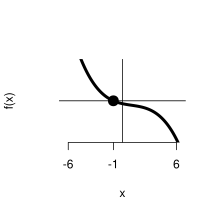
\includegraphics{unnamed-chunk-2-1.pdf}\\
\end{solution}

